% AUTO-GENERADO a partir de Data/Gold/gold_data.json. No editar a mano.
% Paleta categorica (orden fijo, no ciclar) validada para pares adyacentes.
\definecolor{clrblue}{HTML}{2A78D6}
\definecolor{clrorange}{HTML}{EB6834}
\definecolor{clraqua}{HTML}{1BAF7A}
\definecolor{clryellow}{HTML}{EDA100}
\definecolor{clrmagenta}{HTML}{E87BA4}
\definecolor{clrgreen}{HTML}{008300}
\definecolor{clrviolet}{HTML}{4A3AA7}
\definecolor{clrred}{HTML}{E34948}
\definecolor{clrgridgray}{HTML}{D8D6D0}
\definecolor{clrmuted}{HTML}{52514E}

\pgfplotsset{compat=1.18}
\pgfplotsset{
  barbase/.style={
    bar width=13pt, width=\textwidth, height=4.6cm,
    axis lines*=left, enlarge x limits=0.14,
    ymajorgrids, major grid style={clrgridgray, thin},
    axis line style={clrmuted}, tick style={clrmuted},
    every axis label/.append style={font=\scriptsize\color{clrmuted}},
    tick label style={font=\scriptsize, text=clrmuted},
    label style={font=\scriptsize},
    legend style={font=\scriptsize, draw=none, fill=none, at={(0.5,-0.32)}, anchor=north, legend columns=-1},
  },
  singlelabels/.style={
    nodes near coords, every node near coord/.append style={font=\scriptsize, text=black},
  },
  hbarbase/.style={
    xbar, bar width=7pt, width=\textwidth, axis lines*=left,
    xmajorgrids, major grid style={clrgridgray, thin},
    axis line style={clrmuted}, tick style={clrmuted},
    tick label style={font=\scriptsize, text=clrmuted},
    nodes near coords, every node near coord/.append style={font=\tiny, text=black},
    enlarge y limits=0.09,
  },
  linebase/.style={
    width=\textwidth, height=4.6cm, axis lines*=left,
    ymajorgrids, major grid style={clrgridgray, thin},
    axis line style={clrmuted}, tick style={clrmuted},
    tick label style={font=\scriptsize, text=clrmuted},
    legend style={font=\scriptsize, draw=none, fill=none, at={(0.5,-0.30)}, anchor=north, legend columns=-1},
    mark size=1.6pt, thick,
  },
}

\newcommand{\Institucion}{Universidad Distrital Francisco José de Caldas}
\newcommand{\Programa}{Maestria En Ciencias De La Informacion Y Las Comunicaciones}
\newcommand{\Facultad}{Ingeniería}
\newcommand{\NumFactoresTotal}{24}
\newcommand{\NumOportunidades}{20}
\newcommand{\NumFortalezas}{4}
\newcommand{\PesoPromInv}{7.25}
\newcommand{\PesoPromProf}{7.25}
\newcommand{\RCInv}{Resolución 16163 05 SEP 2023}
\newcommand{\RCProf}{Resolución 9925 21 JUN 2023}
\newcommand{\RCVigInv}{7 AÑOS}
\newcommand{\RCVigProf}{7 AÑOS}
\newcommand{\AACInv}{24858 30 DIC 2022}
\newcommand{\AACProf}{24858 30 DIC 2022}
\newcommand{\AACVigInv}{4 AÑOS}
\newcommand{\AACVigProf}{4 AÑOS}
\newcommand{\FechaPlan}{2026-2027}

\newcommand{\ChartFactoresTipo}{
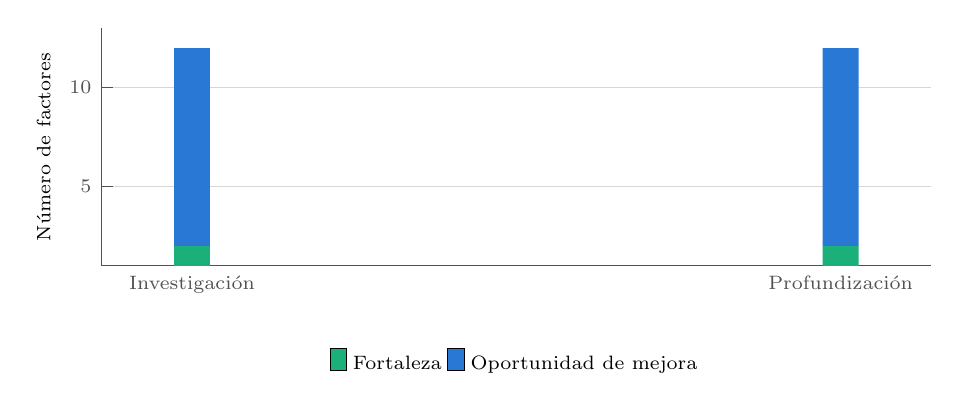
\begin{tikzpicture}
\pgfplotstableread[row sep=\\, col sep=&]{
cat & s0 & s1 \\
0 & 2 & 10 \\
1 & 2 & 10 \\
}\datatable
\begin{axis}[barbase, ybar stacked, xtick={0,1}, xticklabels={Investigación,Profundización}, ylabel={Número de factores}]
\addplot[fill=clraqua, draw=none] table[x=cat, y=s0] {\datatable};
\addplot[fill=clrblue, draw=none] table[x=cat, y=s1] {\datatable};
\legend{Fortaleza,Oportunidad de mejora}
\end{axis}
\end{tikzpicture}
}

\newcommand{\ChartFactoresActividad}{
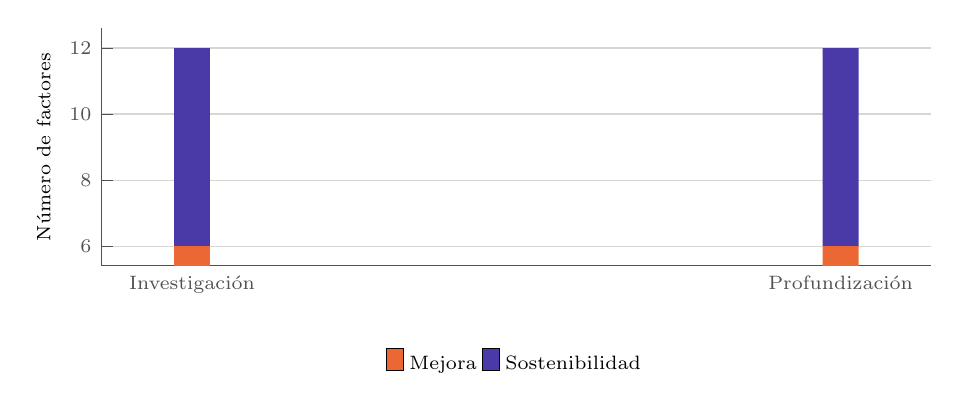
\begin{tikzpicture}
\pgfplotstableread[row sep=\\, col sep=&]{
cat & s0 & s1 \\
0 & 6 & 6 \\
1 & 6 & 6 \\
}\datatable
\begin{axis}[barbase, ybar stacked, xtick={0,1}, xticklabels={Investigación,Profundización}, ylabel={Número de factores}]
\addplot[fill=clrorange, draw=none] table[x=cat, y=s0] {\datatable};
\addplot[fill=clrviolet, draw=none] table[x=cat, y=s1] {\datatable};
\legend{Mejora,Sostenibilidad}
\end{axis}
\end{tikzpicture}
}

\newcommand{\ChartPesoFactores}{
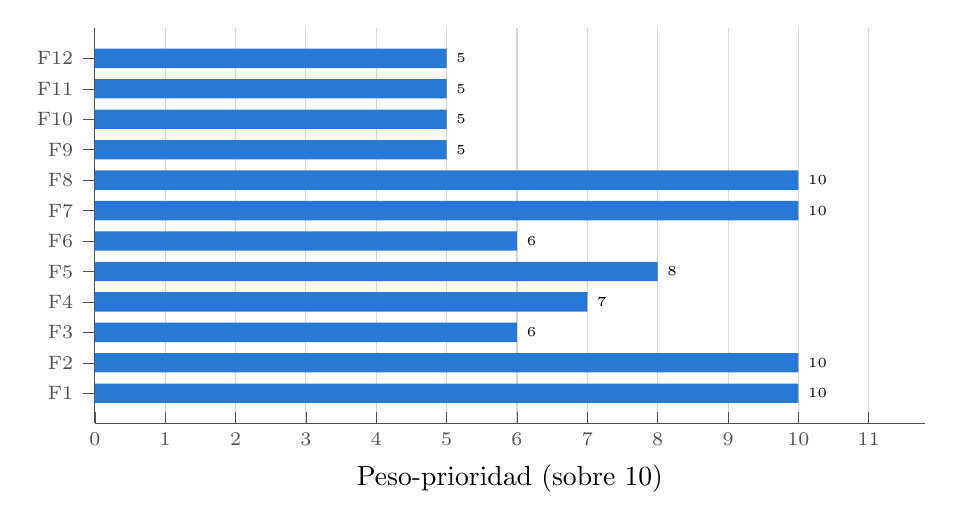
\begin{tikzpicture}
\begin{axis}[hbarbase, height=6.6cm, width=\textwidth, symbolic y coords={F1,F2,F3,F4,F5,F6,F7,F8,F9,F10,F11,F12}, ytick=data, xlabel={Peso-prioridad (sobre 10)}, xmin=0, xmax=11.8]
\addplot[fill=clrblue, draw=none] coordinates {(10,F1) (10,F2) (6,F3) (7,F4) (8,F5) (6,F6) (10,F7) (10,F8) (5,F9) (5,F10) (5,F11) (5,F12)};
\end{axis}
\end{tikzpicture}
}

\newcommand{\TablaFactores}{
\begin{tabular}{@{}c c c p{5.6cm}@{}}
\toprule
\textbf{Factor} & \textbf{Tipo} & \textbf{Peso} & \textbf{Proyecto de mejora} \\
\midrule
1 & Oport. mejora & 10 & Estrategia de socialización y apropiación del PEP y del sistema de… \\
2 & Oport. mejora & 10 & Estrategia de divulgación, acompañamiento y fortalecimiento de comp… \\
3 & Oport. mejora & 6 & Procesos Institucionales Capacitación permanente del equipo docente \\
4 & Fortaleza & 7 & Estrategia de seguimiento, comunicación y evaluación del impacto de… \\
5 & Oport. mejora & 8 & Actualización curricular y fortalecimiento de la retroalimentación… \\
6 & Oport. mejora & 6 & Estrategia de flexibilización curricular y acompañamiento para la g… \\
7 & Oport. mejora & 10 & Cooperación interinstitucional de orden Nacional e internacional de… \\
8 & Fortaleza & 10 & Fortalecimiento de la producción académica y la articulación instit… \\
9 & Oport. mejora & 5 & Estrategia de articulación y divulgación de Bienestar Institucional… \\
10 & Oport. mejora & 5 & Medios educativos y ambientes de aprendizaje en las Maestrías en In… \\
11 & Oport. mejora & 5 & Sistema Interno de Aseguramiento de la Calidad \\
12 & Oport. mejora & 5 & Estrategia de articulación institucional y seguimiento al fortaleci… \\
\bottomrule
\end{tabular}
}

\newcommand{\ChartEnfasis}{
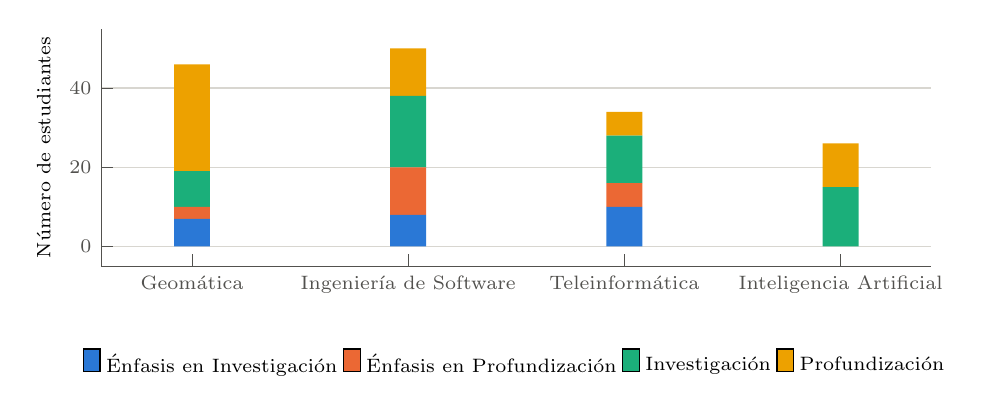
\begin{tikzpicture}
\pgfplotstableread[row sep=\\, col sep=&]{
cat & s0 & s1 & s2 & s3 \\
0 & 7 & 3 & 9 & 27 \\
1 & 8 & 12 & 18 & 12 \\
2 & 10 & 6 & 12 & 6 \\
3 & 0 & 0 & 15 & 11 \\
}\datatable
\begin{axis}[barbase, ybar stacked, xtick={0,1,2,3}, xticklabels={Geomática,Ingeniería de Software,Teleinformática,Inteligencia Artificial}, ylabel={Número de estudiantes}]
\addplot[fill=clrblue, draw=none] table[x=cat, y=s0] {\datatable};
\addplot[fill=clrorange, draw=none] table[x=cat, y=s1] {\datatable};
\addplot[fill=clraqua, draw=none] table[x=cat, y=s2] {\datatable};
\addplot[fill=clryellow, draw=none] table[x=cat, y=s3] {\datatable};
\legend{Énfasis en Investigación,Énfasis en Profundización,Investigación,Profundización}
\end{axis}
\end{tikzpicture}
}

\newcommand{\EnfasisTotalGeneral}{156}
\newcommand{\NumEnfasis}{4}
\newcommand{\TablaEnfasisTotales}{
\begin{tabular}{@{}l r@{}}
\toprule
\textbf{\'Enfasis} & \textbf{Estudiantes activos} \\
\midrule
Geomática & 46 \\
Ingeniería de Software & 50 \\
Teleinformática & 34 \\
Inteligencia Artificial & 26 \\
\midrule
\textbf{Total} & \textbf{156} \\
\bottomrule
\end{tabular}
}

\newcommand{\ChartEstadoAcademico}{
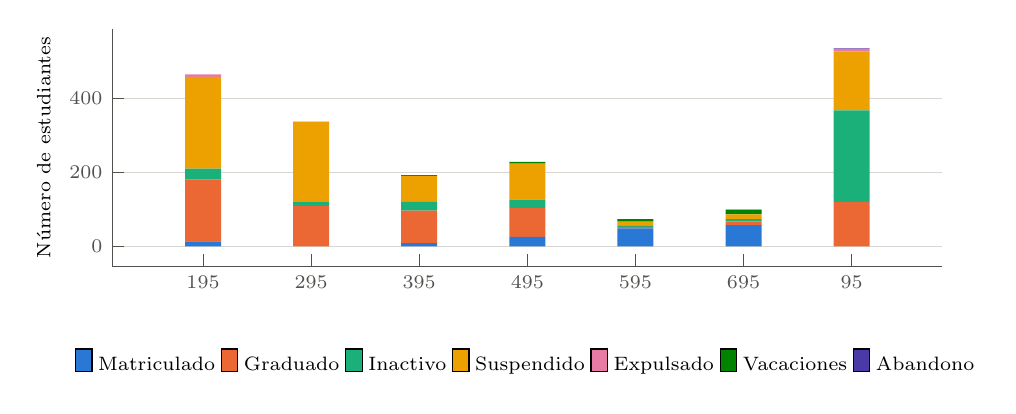
\begin{tikzpicture}
\pgfplotstableread[row sep=\\, col sep=&]{
cat & s0 & s1 & s2 & s3 & s4 & s5 & s6 \\
0 & 14 & 167 & 30 & 248 & 7 & 0 & 0 \\
1 & 0 & 109 & 11 & 217 & 1 & 0 & 0 \\
2 & 9 & 88 & 24 & 70 & 0 & 2 & 0 \\
3 & 26 & 78 & 23 & 97 & 0 & 5 & 0 \\
4 & 49 & 4 & 4 & 10 & 0 & 7 & 0 \\
5 & 58 & 10 & 6 & 13 & 0 & 12 & 1 \\
6 & 0 & 121 & 247 & 159 & 8 & 0 & 1 \\
}\datatable
\begin{axis}[barbase, ybar stacked, xtick={0,1,2,3,4,5,6}, xticklabels={195,295,395,495,595,695,95}, ylabel={Número de estudiantes}]
\addplot[fill=clrblue, draw=none] table[x=cat, y=s0] {\datatable};
\addplot[fill=clrorange, draw=none] table[x=cat, y=s1] {\datatable};
\addplot[fill=clraqua, draw=none] table[x=cat, y=s2] {\datatable};
\addplot[fill=clryellow, draw=none] table[x=cat, y=s3] {\datatable};
\addplot[fill=clrmagenta, draw=none] table[x=cat, y=s4] {\datatable};
\addplot[fill=clrgreen, draw=none] table[x=cat, y=s5] {\datatable};
\addplot[fill=clrviolet, draw=none] table[x=cat, y=s6] {\datatable};
\legend{Matriculado,Graduado,Inactivo,Suspendido,Expulsado,Vacaciones,Abandono}
\end{axis}
\end{tikzpicture}
}

\newcommand{\TotalEstudiantesHistorico}{1936}
\newcommand{\TablaProyectosCurriculares}{
\begin{tabular}{@{}c p{5.4cm} r@{}}
\toprule
\textbf{C\'od.} & \textbf{Proyecto curricular} & \textbf{Total} \\
\midrule
195 & MAE. EN CIENCIAS DE LA INF. Y LAS COMUNICACIONES ENFASIS… & 466 \\
295 & MAE. EN CIENCIAS DE LA INF. Y LAS COMUNICACIONES ENFASIS… & 338 \\
395 & MAE. EN CIENCIAS DE LA INF. Y LAS COMUNICACIONES ENFASIS… & 193 \\
495 & MAE. EN CIENCIAS DE LA INF. Y LAS COMUNICACIONES ENFASIS… & 229 \\
595 & MAESTRÍA EN CIENCIAS DE LA INFORMACIÓN Y LAS COMUNICACION… & 74 \\
695 & MAESTRÍA EN CIENCIAS DE LA INFORMACIÓN Y LAS COMUNICACION… & 100 \\
95 & MAESTRIA EN TELEINFORMATICA & 536 \\
\bottomrule
\end{tabular}
}

\newcommand{\ChartEgresadosAnio}{
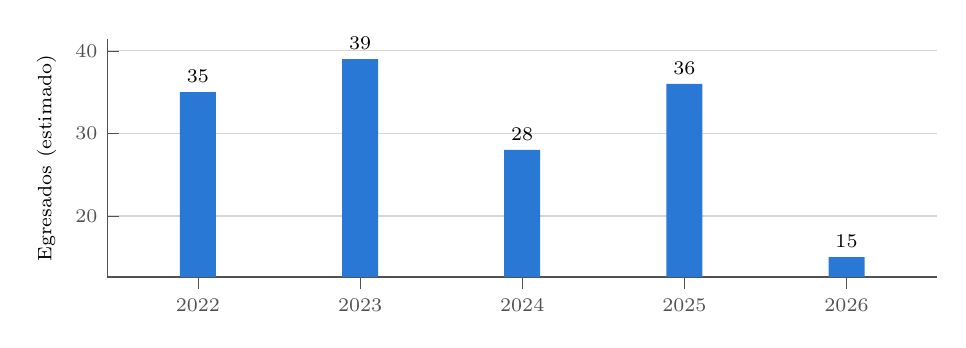
\begin{tikzpicture}
\begin{axis}[barbase, ybar, singlelabels, height=4.6cm, symbolic x coords={2022,2023,2024,2025,2026}, xtick=data, ylabel={Egresados (estimado)}]
\addplot[fill=clrblue, draw=none] coordinates {(2022,35) (2023,39) (2024,28) (2025,36) (2026,15)};
\end{axis}
\end{tikzpicture}
}

\newcommand{\TotalEgresadosHistorico}{577}
\newcommand{\RangoEgresados}{2022-2026}
\newcommand{\ChartEgresadosProyecto}{
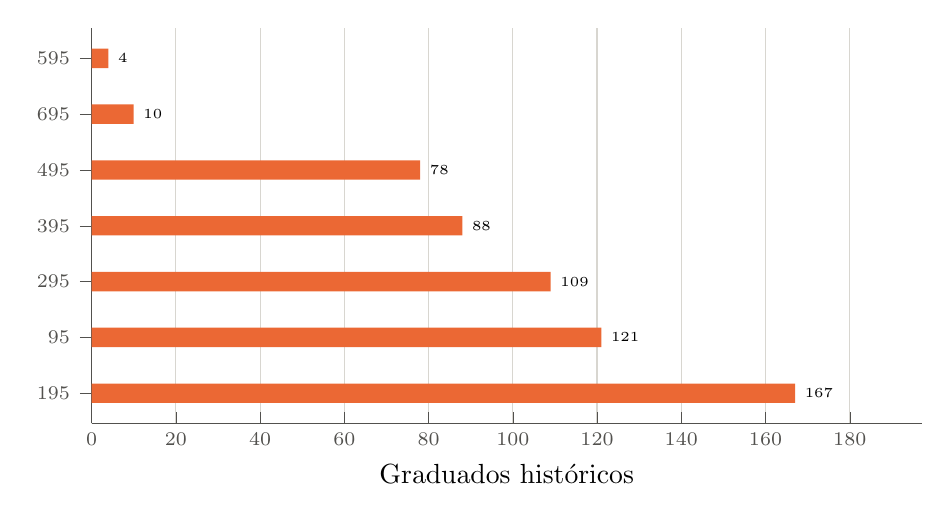
\begin{tikzpicture}
\begin{axis}[hbarbase, height=6.6cm, width=\textwidth, symbolic y coords={195,95,295,395,495,695,595}, ytick=data, xlabel={Graduados hist\'oricos}, xmin=0, xmax=197.1]
\addplot[fill=clrorange, draw=none] coordinates {(167,195) (121,95) (109,295) (88,395) (78,495) (10,695) (4,595)};
\end{axis}
\end{tikzpicture}
}

\newcommand{\ChartEgresadosFechaReal}{
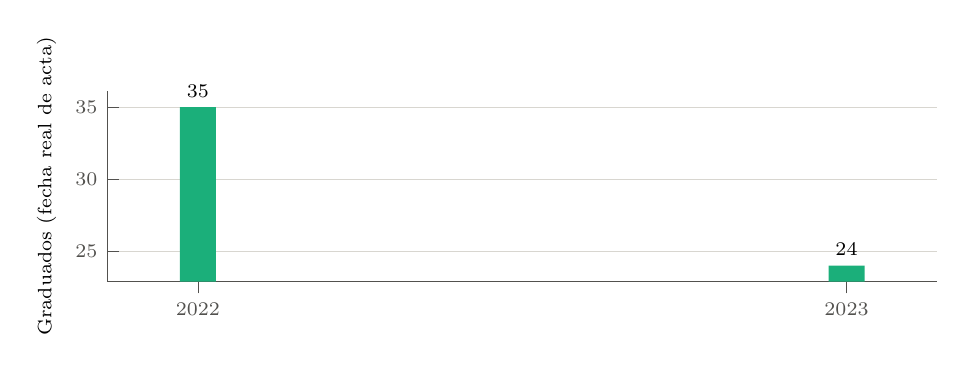
\begin{tikzpicture}
\begin{axis}[barbase, ybar, singlelabels, height=4.0cm, symbolic x coords={2022,2023}, xtick=data, ylabel={Graduados (fecha real de acta)}]
\addplot[fill=clraqua, draw=none] coordinates {(2022,35) (2023,24)};
\end{axis}
\end{tikzpicture}
}
\newcommand{\TotalEgresadosFechaReal}{59}
\newcommand{\RangoFechaReal}{2022-2023}
\newcommand{\ValidacionCoinciden}{59}
\newcommand{\ValidacionComparables}{59}

\newcommand{\ChartGruposClasificacion}{
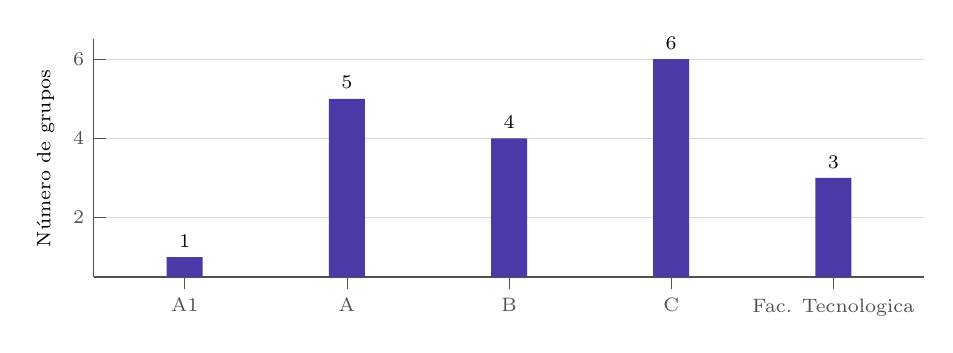
\begin{tikzpicture}
\begin{axis}[barbase, ybar, singlelabels, height=4.6cm, symbolic x coords={A1,A,B,C,Fac. Tecnologica}, xtick=data, ylabel={Número de grupos}]
\addplot[fill=clrviolet, draw=none] coordinates {(A1,1) (A,5) (B,4) (C,6) (Fac. Tecnologica,3)};
\end{axis}
\end{tikzpicture}
}

\newcommand{\NumGrupos}{25}
\newcommand{\NumDocentesGrupos}{87}
\newcommand{\NumProyectosConGrupo}{414}
\newcommand{\TablaGruposUno}{
\begin{tabular}{@{}l c p{4.0cm} c c@{}}
\toprule
\textbf{Sigla} & \textbf{Clasif.} & \textbf{L\'ider} & \textbf{Docentes} & \textbf{Proy.} \\
\midrule
GCEM & C & Edwin Rivas Trujillo & 4 & 1 \\
GEFEM & C & Luis Eduardo Castillo Méndez & 4 & 40 \\
GESETIC & C & Alvaro Espinel Ortega & 4 & 15 \\
GICOECOL & B & José Ignacio Rodríguez Molano & 2 & 2 \\
GICOGE & C & José Nelson Pérez Castillo & 8 & 37 \\
GIIRA & A1 & Carlos Enrique Montenegro Marín & 6 & 43 \\
GITUD & C & Elvis Eduardo Gaona García & 6 & 9 \\
GITEM++ & B & Lilia Edith Aparicio Pico & 5 & 35 \\
GRECO & B & Carlos Arturo Suárez Fajardo & 3 & 8 \\
Internet Inteligente & A & Octavio Salcedo Parra & 4 & 39 \\
\bottomrule
\end{tabular}
}

\newcommand{\TablaGruposDos}{
\begin{tabular}{@{}l c p{4.0cm} c c@{}}
\toprule
\textbf{Sigla} & \textbf{Clasif.} & \textbf{L\'ider} & \textbf{Docentes} & \textbf{Proy.} \\
\midrule
INTECSE & A & Julio Barón Velandia & 2 & 24 \\
ITI & Fac.Tecn. & Hector Florez & 1 & 11 \\
LAMIC & C & Andrés Eduardo Gaona Barrera & 4 & 11 \\
LASER & B & Ernesto Gómez Vargas & 6 & 39 \\
LIDER & A & Roberto Ferro Escobar & 3 & 26 \\
LIFAE & A & Nelson Díaz Aldana & 3 & 2 \\
NIDE & A & Luz Ángela Rocha Salamanca & 13 & 70 \\
ARMOS & Fac.Tecn. & - & 0 & 1 \\
GIDENUTAS & Fac.Tecn. & - & 0 & 1 \\
\bottomrule
\end{tabular}
}

\newcommand{\ChartProduccionGrupos}{
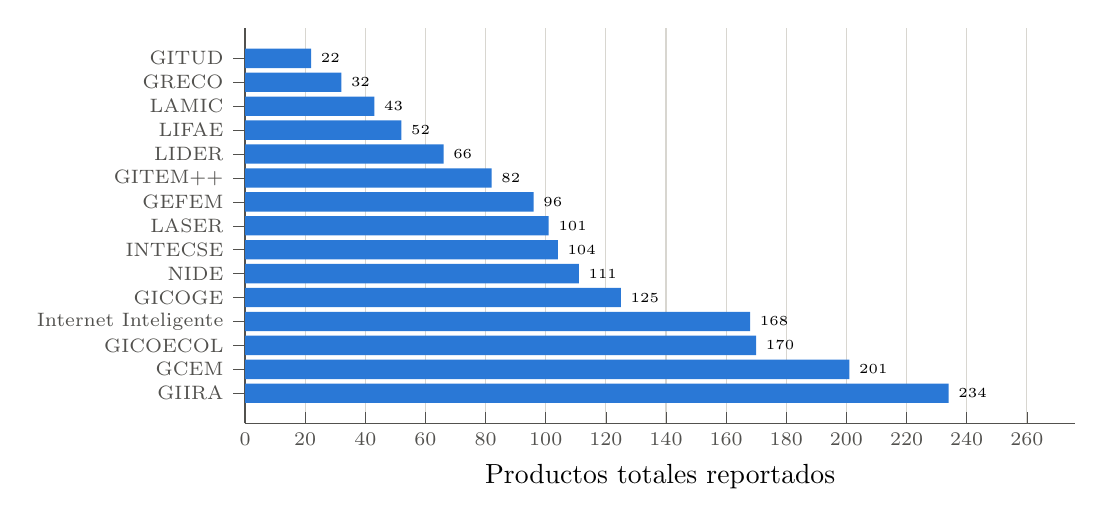
\begin{tikzpicture}
\begin{axis}[hbarbase, height=6.6cm, width=\textwidth, symbolic y coords={GIIRA,GCEM,GICOECOL,Internet Inteligente,GICOGE,NIDE,INTECSE,LASER,GEFEM,GITEM++,LIDER,LIFAE,LAMIC,GRECO,GITUD}, ytick=data, xlabel={Productos totales reportados}, xmin=0, xmax=276.1]
\addplot[fill=clrblue, draw=none] coordinates {(234,GIIRA) (201,GCEM) (170,GICOECOL) (168,Internet Inteligente) (125,GICOGE) (111,NIDE) (104,INTECSE) (101,LASER) (96,GEFEM) (82,GITEM++) (66,LIDER) (52,LIFAE) (43,LAMIC) (32,GRECO) (22,GITUD)};
\end{axis}
\end{tikzpicture}
}

\newcommand{\NumGruposProduccion}{15}
\newcommand{\TotalProductosGrupos}{1607}
\newcommand{\ChartTesisEtapa}{
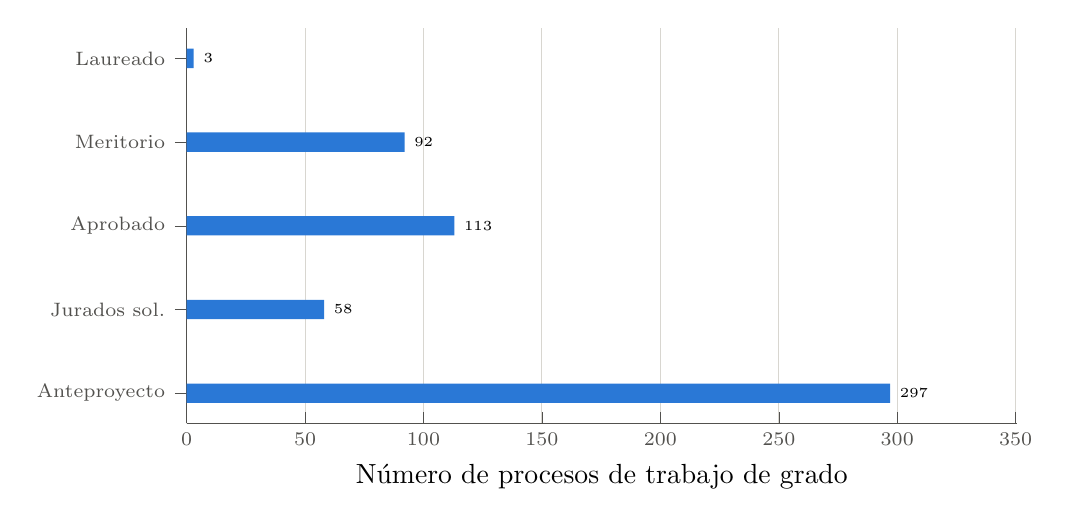
\begin{tikzpicture}
\begin{axis}[hbarbase, height=6.6cm, width=\textwidth, symbolic y coords={Anteproyecto,Jurados sol.,Aprobado,Meritorio,Laureado}, ytick=data, xlabel={Número de procesos de trabajo de grado}, xmin=0, xmax=350.5]
\addplot[fill=clrblue, draw=none] coordinates {(297,Anteproyecto) (58,Jurados sol.) (113,Aprobado) (92,Meritorio) (3,Laureado)};
\end{axis}
\end{tikzpicture}
}

\newcommand{\TotalProcesosTesis}{563}
\newcommand{\NumSinGrupo}{149}
\newcommand{\NumConGrupo}{25}
\newcommand{\ChartTesisModalidad}{
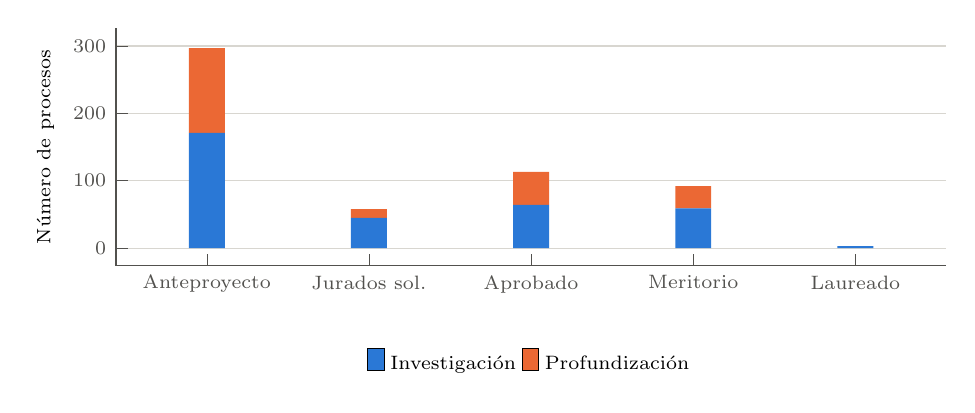
\begin{tikzpicture}
\pgfplotstableread[row sep=\\, col sep=&]{
cat & s0 & s1 \\
0 & 171 & 126 \\
1 & 45 & 13 \\
2 & 64 & 49 \\
3 & 59 & 33 \\
4 & 3 & 0 \\
}\datatable
\begin{axis}[barbase, ybar stacked, xtick={0,1,2,3,4}, xticklabels={Anteproyecto,Jurados sol.,Aprobado,Meritorio,Laureado}, ylabel={Número de procesos}]
\addplot[fill=clrblue, draw=none] table[x=cat, y=s0] {\datatable};
\addplot[fill=clrorange, draw=none] table[x=cat, y=s1] {\datatable};
\legend{Investigación,Profundización}
\end{axis}
\end{tikzpicture}
}

\newcommand{\TotalTesisInv}{342}
\newcommand{\TotalTesisProf}{221}
\newcommand{\ChartCNAMatriculados}{
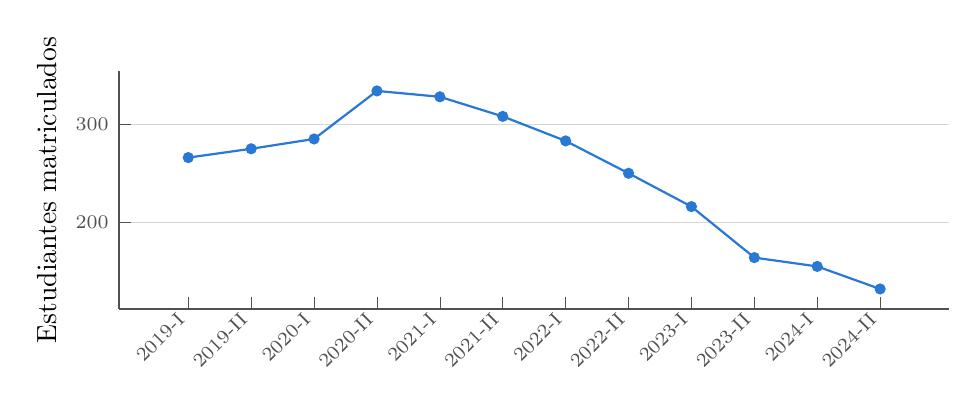
\begin{tikzpicture}
\begin{axis}[linebase, symbolic x coords={2019-I,2019-II,2020-I,2020-II,2021-I,2021-II,2022-I,2022-II,2023-I,2023-II,2024-I,2024-II}, xtick=data, x tick label style={rotate=45,anchor=east}, ylabel={Estudiantes matriculados}]
\addplot[color=clrblue, mark=*] coordinates {(2019-I,266) (2019-II,275) (2020-I,285) (2020-II,334) (2021-I,328) (2021-II,308) (2022-I,283) (2022-II,250) (2023-I,216) (2023-II,164) (2024-I,155) (2024-II,132)};
\end{axis}
\end{tikzpicture}
}

\newcommand{\ChartCNAGraduados}{
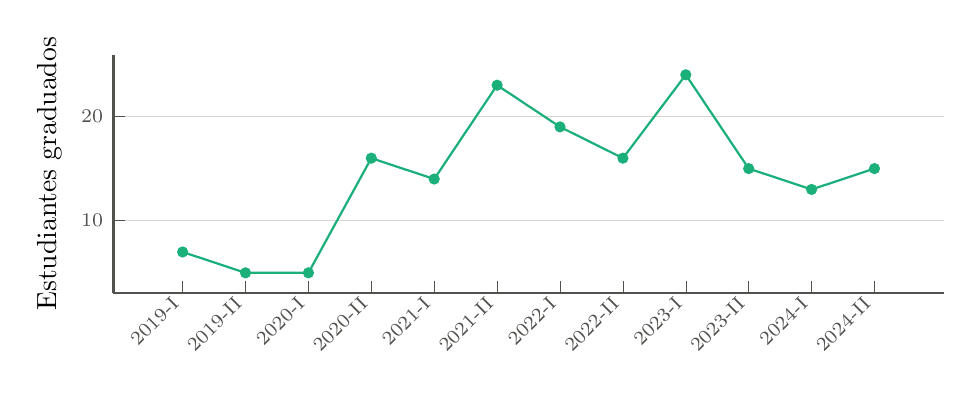
\begin{tikzpicture}
\begin{axis}[linebase, symbolic x coords={2019-I,2019-II,2020-I,2020-II,2021-I,2021-II,2022-I,2022-II,2023-I,2023-II,2024-I,2024-II}, xtick=data, x tick label style={rotate=45,anchor=east}, ylabel={Estudiantes graduados}]
\addplot[color=clraqua, mark=*] coordinates {(2019-I,7) (2019-II,5) (2020-I,5) (2020-II,16) (2021-I,14) (2021-II,23) (2022-I,19) (2022-II,16) (2023-I,24) (2023-II,15) (2024-I,13) (2024-II,15)};
\end{axis}
\end{tikzpicture}
}

\newcommand{\ChartBienestar}{
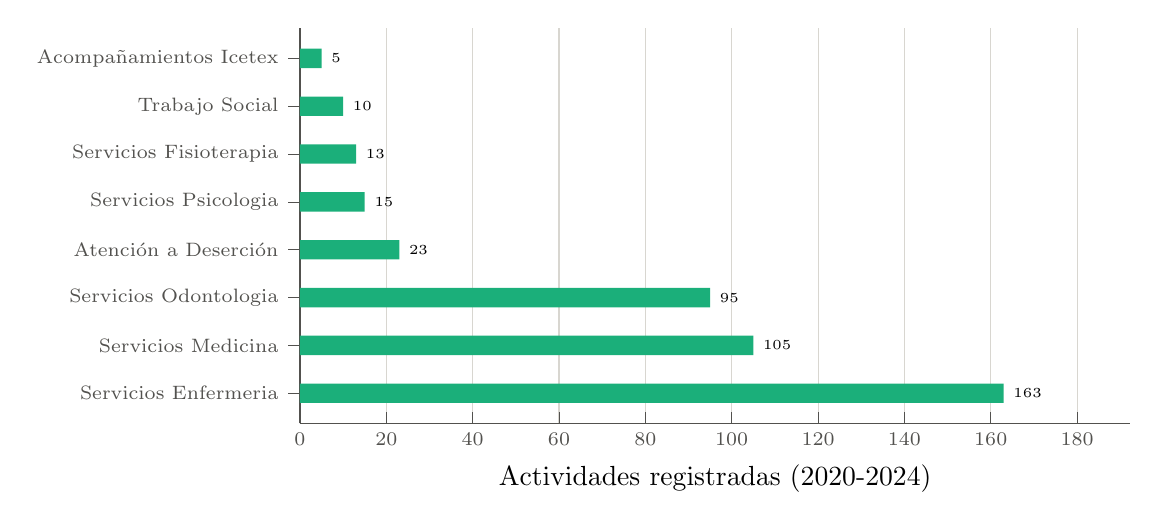
\begin{tikzpicture}
\begin{axis}[hbarbase, height=6.6cm, width=\textwidth, symbolic y coords={Servicios Enfermeria,Servicios Medicina,Servicios Odontologia,Atención a Deserción,Servicios Psicologia,Servicios Fisioterapia,Trabajo Social,Acompañamientos Icetex}, ytick=data, xlabel={Actividades registradas (2020-2024)}, xmin=0, xmax=192.3]
\addplot[fill=clraqua, draw=none] coordinates {(163,Servicios Enfermeria) (105,Servicios Medicina) (95,Servicios Odontologia) (23,Atención a Deserción) (15,Servicios Psicologia) (13,Servicios Fisioterapia) (10,Trabajo Social) (5,Acompañamientos Icetex)};
\end{axis}
\end{tikzpicture}
}

\newcommand{\ChartDocsExtension}{
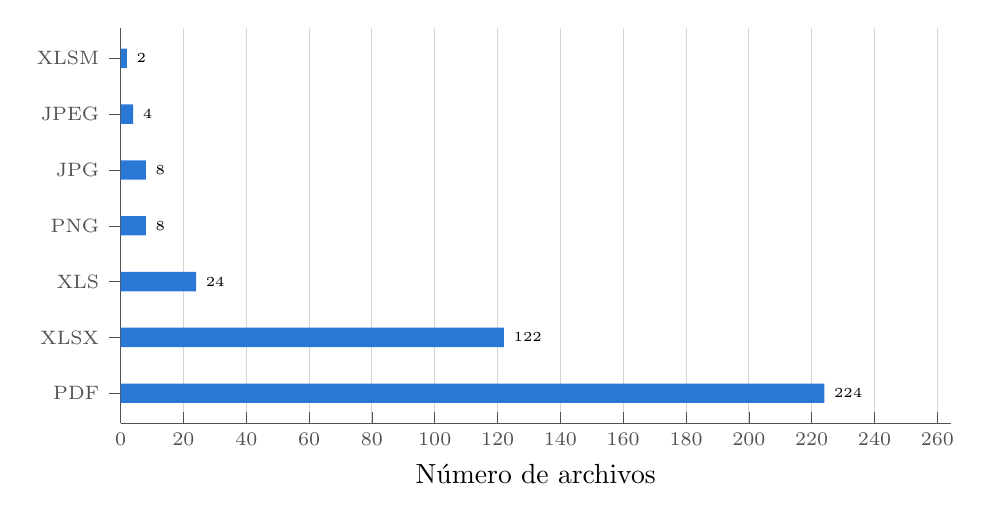
\begin{tikzpicture}
\begin{axis}[hbarbase, height=6.6cm, width=\textwidth, symbolic y coords={PDF,XLSX,XLS,PNG,JPG,JPEG,XLSM}, ytick=data, xlabel={Número de archivos}, xmin=0, xmax=264.3]
\addplot[fill=clrblue, draw=none] coordinates {(224,PDF) (122,XLSX) (24,XLS) (8,PNG) (8,JPG) (4,JPEG) (2,XLSM)};
\end{axis}
\end{tikzpicture}
}

\newcommand{\ChartDocsModalidad}{
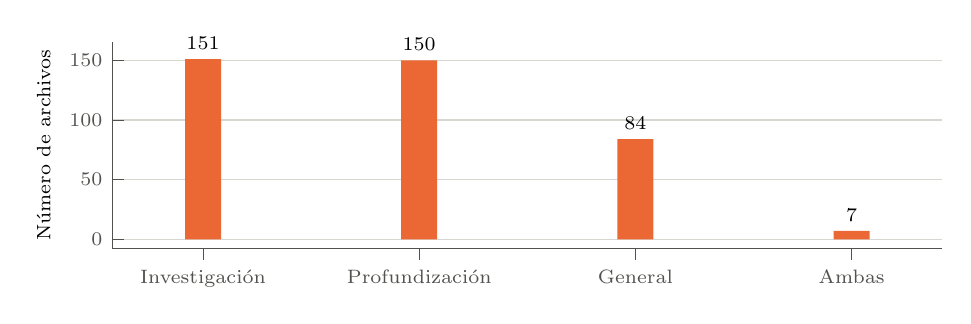
\begin{tikzpicture}
\begin{axis}[barbase, ybar, singlelabels, height=4.2cm, symbolic x coords={Investigación,Profundización,General,Ambas}, xtick=data, ylabel={Número de archivos}]
\addplot[fill=clrorange, draw=none] coordinates {(Investigación,151) (Profundización,150) (General,84) (Ambas,7)};
\end{axis}
\end{tikzpicture}
}

\newcommand{\ChartDocsCarpeta}{
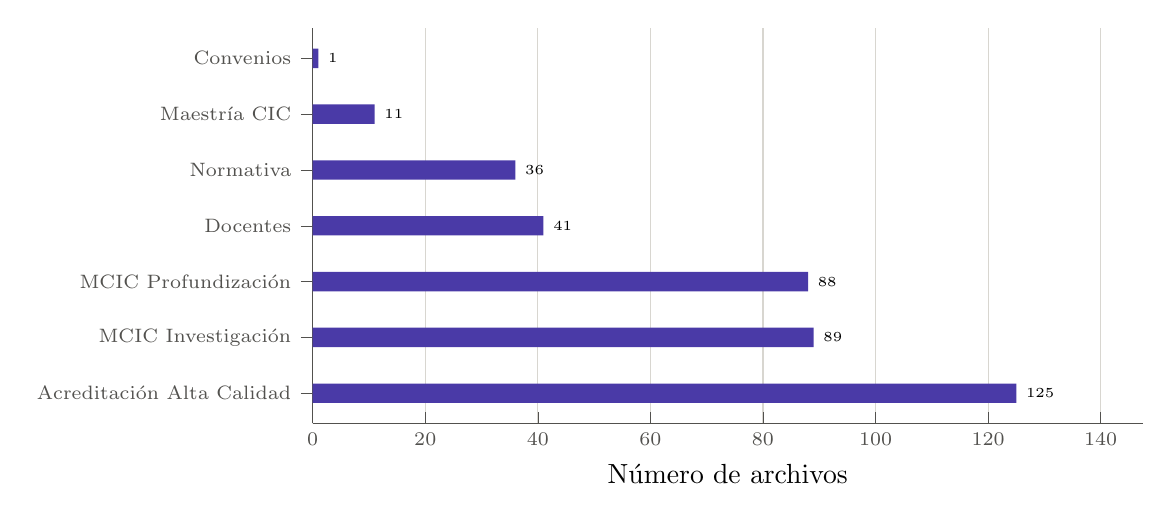
\begin{tikzpicture}
\begin{axis}[hbarbase, height=6.6cm, width=\textwidth, symbolic y coords={Acreditación Alta Calidad,MCIC Investigación,MCIC Profundización,Docentes,Normativa,Maestría CIC,Convenios}, ytick=data, xlabel={Número de archivos}, xmin=0, xmax=147.5]
\addplot[fill=clrviolet, draw=none] coordinates {(125,Acreditación Alta Calidad) (89,MCIC Investigación) (88,MCIC Profundización) (41,Docentes) (36,Normativa) (11,Maestría CIC) (1,Convenios)};
\end{axis}
\end{tikzpicture}
}

\newcommand{\TotalDocsBronze}{392}
\newcommand{\TotalDocsConTexto}{309}
\newcommand{\PctDocsConTexto}{79}
